% **************************************************
% Document class
% **************************************************
% cSpell:disable
\documentclass[
    a4paper,
    12pt,
    bibliography=totoc,
    listof=totoc,
    titlepage,
    footheight=19.28502pt,
    headsepline  % Thêm đường gạch chân cho tiêu đề
]{scrartcl}

% **************************************************
% Settings
% **************************************************

\usepackage{settings}
\usepackage{bookmark}
% Tùy chỉnh tiêu đề trang
%\usepackage[automark]{scrlayer-scrpage}
%\clearpairofpagestyles
%\chead{\upshape\headmark} % Tiêu đề ở giữa, không nghiêng
%%\ohead{\pagemark} % Số trang ở góc ngoài bên phải

% Đặt font chữ thẳng cho tiêu đề
%\setkomafont{pageheadfoot}{\normalfont}
%\setkomafont{pagenumber}{\normalfont}

% Tùy chỉnh tiêu đề trang (nếu cần)
\renewcommand{\sectionmark}[1]{\markboth{#1}{}}
\renewcommand{\subsectionmark}[1]{\markright{#1}}
\renewcommand{\figurename}{Abbildung}

% **************************************************
% Additional Biblatex configuration
% **************************************************
\DeclareNameAlias{sortname}{family-given}
\DeclareDelimFormat{nameyeardelim}{\addcomma\space}

% **************************************************
% Variables
% **************************************************

\newcommand*{\getUniversity}{Hochschule für angewandte Wissenschaften München}
\newcommand*{\getFaculty}{Fakultät für Informatik und Mathematik}
\newcommand*{\getTitle}{Integration von Climate Risk und Geospatial Analyse zur Risikobewertung von Immobilienportfolios}
\newcommand*{\getAuthor}{Uyen Truong}
\newcommand*{\getCourse}{Stochastic Engineering in Business and Finance}
\newcommand*{\getDoctype}{Masterarbeit}
\newcommand*{\getSupervisor}{Prof. Dr. Silja Grawert}
\newcommand*{\getSubmissionDate}{\today}

% **************************************************
% Content
% **************************************************

\begin{document}

\thispagestyle{empty}

% Logo oben rechteckig
\begin{flushright}

\includegraphics[width=6cm,keepaspectratio]{logos/university_logo}
\end{flushright}

\vspace*{1cm}

% Obere Linie
\noindent\rule{\linewidth}{0.5mm}

\vspace{1cm}

% Titel
\begin{flushright}
  \sffamily\bfseries\LARGE
  \getTitle
  
  \vspace{0.5cm}
  
  {\Large\getAuthor}
\end{flushright}

\vspace{1cm}

% Untere Linie
\noindent\rule{\linewidth}{0.5mm}

\vspace*{\stretch{1}}

% Zusätzliche Informationen
\begin{center}
  \large
  Masterarbeit\\
  \vspace{0.5cm}
  an der \getUniversity\\
  \getFaculty
  
  \vspace{1cm}
  
  Studienrichtung: \getCourse
  
  \vspace{1cm}
  
  vorgelegt von\\
  \getAuthor
  
  \vspace{\stretch{1}}
  
  München, den \getSubmissionDate
  
  \vspace{1cm}
  
  Erstgutachter: \getSupervisor
\end{center}



\section*{Abstract}
Lorem ipsum dolor sit amet, consetetur sadipscing elitr, sed diam nonumy eirmod tempor invidunt ut labore et dolore magna aliquyam erat, sed diam voluptua. At vero eos et accusam et justo duo dolores et ea rebum. Stet clita kasd gubergren, no sea takimata sanctus est Lorem ipsum dolor sit amet. Lorem ipsum dolor sit amet, consetetur sadipscing elitr, sed diam nonumy eirmod tempor invidunt ut labore et dolore magna aliquyam erat, sed diam voluptua. At vero eos et accusam et justo duo dolores et ea rebum. Stet clita kasd gubergren, no sea takimata sanctus est Lorem ipsum dolor sit amet.



\tableofcontents

\clearpage
\listoffigures

\clearpage
\listoftables

\clearpage
\lstlistoflistings

\clearpage
\section*{Abkürzungsverzeichnis}

\begin{acronym}[CI]

\acro{abc}[ABC]{American Broadcasting Company}

\end{acronym}

\clearpage
\section{Einleitung}

Im Folgenden wird beispielhaft gezeigt, wie Zitate, Bilder, Tabellen oder Quellcode in die Arbeit eingefügt werden können.

\subsection{Zitate}
Menschen, die mit ihrem IQ prahlen, sind Versager.

\subsection{Bilder}
\begin{figure}[H] 
    \centering
    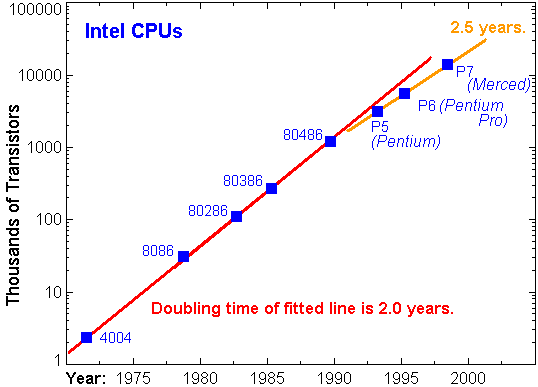
\includegraphics[width=0.5\textwidth]{figures/figure_example.png}
    \caption{Mooresches Gesetz}
\end{figure}

\subsection{Tabellen}
\begin{table}[H]
    \centering
    \begin{tabular}[H]{l|l|l}
        Bezeichnung & Kerne & TDP \\
        \hline
        Intel Core i5 & 6 & 111 W \\
        \hline
        AMD Ryzen 7 & 8 & 178 W \\
    \end{tabular}
    \caption{Prozessoren}
\end{table}


\subsection{Quellcode}
\begin{lstlisting}[language=java, caption=Hello World in Java, captionpos=b]
    class HelloWorld {
        public static void main(String[] args) {
            // Display the string.y
            System.out.println("Hello World!");
        }
    }
\end{lstlisting}


% cSpell:disable
\section{Theoretischer Hintergrund}

\subsection{Wesentliche Begriffe}
\subsubsection{Beleihungsauslauf}
Der Beleihungsauslauf, auch als Loan-to-Value-Ratio bekannt, ist eine zentrale Kennzahl in der Immobilienfinanzierung \parencite{BelWertV_3}. Er wird definiert als:
\begin{equation}
    \text{Beleihungsauslauf} = \frac{\text{Darlehensbetrag}}{\text{Beleihungswert}}
    \label{eq:ltv}
\end{equation}

\noindent wobei:
\begin{itemize}
    \item Der Darlehensbetrag ist die Höhe des Darlehens.
    \item Der Beleihungswert ist der langfristig erzielbare Wert einer Immobilie, unabhängig von kurzfristigen Marktschwankungen.
\end{itemize}

Ein geringerer Beleihungsauslauf zeigt dem Kreditgeber ein reduziertes Risiko für Zahlungsausfälle an. Daraus ergibt sich ein erhöhter Beleihungsauslauf, was zu einem höheren Risiko führt und in der Regel zu weniger günstigen Bedingungen für den Kreditnehmer führt.

Um das Konzept zu verdeutlichen, wird ein Fallbeispiel einer Immobilienfinanzierung betrachtet: Ein Gutachter schätzt den Beleihungswert einer Immobilie auf 500.000 Euro.Die Person, die das Haus kaufen möchte, beantragt ein Darlehen in Höhe von 275.000 Euro. Die Person, die das Haus kaufen möchte, beantragt ein Darlehen von 275.000 Euro.
Der Beleihungsauslauf wird gemäß Gleichung \ref{eq:ltv} folgendermaßen berechnet:
\begin{equation}
    \text{Beleihungsauslauf} = \frac{\text{Darlehensbetrag}}{\text{Beleihungswert}} = \frac{275.000 \mbox{\texteuro}}{500.000 \mbox{\texteuro}} = 0,55 = 55\%
\end{equation}
Der Beleihungsauslauf in diesem Fall beträgt 55\%. Das bedeutet, dass 55\% des Immobilienwertes wird von der Bank finanziert. Die restlichen 45\% müssen durch Eigenkapital oder oder andere Einnahmequellen abgedeckt werden.
\subsubsection{Transitionsrisiken}
Transitionsrisiken bezeichnen das Risiko finanzieller Verluste für Institutionen, die aus dem Anpassungsprozess hin zu einer Wirtschaft mit weniger CO2-Emissionen und einer umweltfreundlicheren Ökonomie entstehen \parencite{ecb2020climate}. Dieses Konzept, das in den Bereichen ESG, Klimawandel, Wirtschaft und Finanzen breite Anwendung findet, umfasst vier Hauptkategorien: Technologie-, Marktpreis-, Regulierungs- und Reputationsrisiken.

Besonders exponiert gegenüber diesen Risiken ist der Immobiliensektor, der für etwa 40\% der globalen Treibhausgasemissionen verantwortlich zeichnet \parencite{unepfi2023realestate} und somit vor erheblichen Anpassungsherausforderungen steht.
Für diesen Sektorentstehen Transitionsrisiken vorwiegend durch regulatorische Änderungen, insbesondere durch neue Gesetze zu Energiepreisen und CO2-Steuern. Diese Entwicklungen zwingen den Sektor zu weitreichenden Anpassungen, um wettbewerbsfähig zu bleiben und gleichzeitig Nachhaltigkeitsziele zu erreichen.
\subsubsection{Physische Risiken}
Unter physischen Risiken versteht man Gefahren, die aus natürlichen Ereignissen oder Umweltbedingungen entstehen und negative Konsequenzen für Gesellschaft, Wirtschaft und Ökosysteme nach sich ziehen können \parencite{greenvisionsolutions_transitorische_2024}. Diese Risiken werden typischerweise in akute Risiken, die durch plötzliche extreme Ereignisse wie Überschwemmungen oder Stürme hervorgerufen werden, und chronische Risiken, die sich aus langfristigen klimatischen Veränderungen wie dem Meeresspiegelanstieg, Wasserstress, Biodiversitätsverlust und Ressourcenknappheit ergeben, unterteilt \parencite{dnb2019values}.

\subsubsection{Klimaszenarien des NGFS}
Das \ac{NGFS} hat 72 verschiedene Klimaszenarien entwickelt, wovon sechs für diese Arbeit ausgewählt wurden. Diese sechs Szenarien repräsentieren ein breites Spektrum möglicher Entwicklungen unter Berücksichtigung verschiedener physischer Risiken und Transitionsrisiken. In Abbildung \ref{fig:ngfs} ist die Darstellung der sechs Haupt-Szenarien des NGFS im Rahmenwerk zu sehen. In Tabelle \ref{tab:ngfs-framework} sind ausführliche Erläuterungen zu diesen Situationen enthalten.

\begin{figure}[htbp]
    \centering
    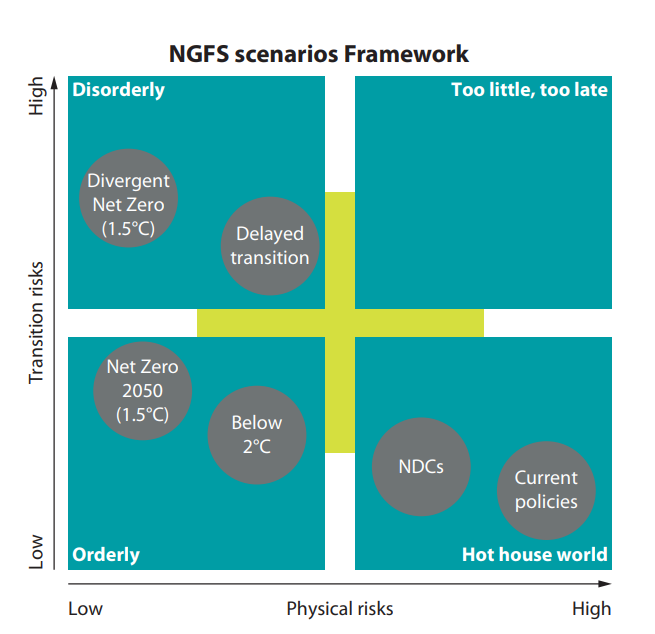
\includegraphics[width=0.7\textwidth]{figures/NGFS.png}
    \caption{NGFS Klimaszenario-Framework. Quelle: NGFS Climate Scenarios for central banks and supervisors (June 2021)}
    \label{fig:ngfs}
\end{figure}
\FloatBarrier

\begin{table}[htbp]
    \centering
    \small
    \caption{Überblick über NGFS-Rahmen zur Klassifizierung von Klimarisiken. In Anlehnung an Quelle: NGFS Climate Scenarios for central banks and supervisors (June 2021).}
    \label{tab:ngfs-framework}
    \begin{tabularx}{1.0\textwidth}{>{\raggedright\arraybackslash}X >{\centering\arraybackslash}X >{\centering\arraybackslash}X >{\raggedright\arraybackslash}X}
        \toprule
        \textbf{Szenario} & \textbf{Transitionsrisiken} & \textbf{Physische Risiken} & \textbf{Beschreibung} \\
        \midrule
        Orderly & Niedrig & Niedrig & Frühzeitige Einführung von Klimapolitiken, die allmählich strenger werden. Keine wesentlichen Diskrepanzen zwischen Politiken. \\
        \addlinespace
        Disorderly & Hoch & Niedrig & Höhere Transitionsrisiken aufgrund verzögerter oder inkonsistenter Klimapolitiken. Sehr strenge Politiken bei Einführung. \\
        \addlinespace
        Hot house world & Niedrig & Hoch & Nur wenige Länder führen Klimapolitiken ein. Globale Bemühungen unzureichend, führt zu irreversiblen Auswirkungen. \\
        \addlinespace
        Too little, too late & Hoch & Hoch & Extremste Szenarien. Unzureichende Maßnahmen führen zu Katastrophen und erzwingen einen ungeordneten Übergang. \\
        \bottomrule
    \end{tabularx}
\end{table}
\FloatBarrier

Die Szenarien "`Orderly"', "`Disorderly"' und "`Hot House World"' für die Jahre 2030, 2040 und 2050 stehen im Mittelpunkt. Im EZB-Klimarisiko-Stresstest werden sie mittels eines Bottom-up-Ansatzes berücksichtigt und beinhalten sowohl Transitions- als auch physische
Risiken. Diese Szenarien bilden die Grundlage für die Analyse der potenziellen Auswirkungen verschiedener Klimapolitiken auf den Immobiliensektor über einen längeren Zeitraum und ermöglichen eine detaillierte Untersuchung der Bruttowertschöpfung in diesem Sektor.

\subsubsection{Abflussmenge bei Hochwasser}\label{sec:HQ}

Die Festlegung von Hochwasserrisikogebieten in Deutschland erfolgt gesetzlich anhand der Anzahl von HQ\textsubscript{T\textsubscript{n} }-Ereignissen gemäß dem \textcite{WHG73}. Hierbei steht HQ für die Abflussmenge bei Hochwasser, während T\textsubscript{n} für den statistische Wiederkehrperiode des Ereignisses. Beispielsweise bezeichnet ein HQ\textsubscript{100} ein statistisch einmal in 100 Jahren auftretendes Hochwasserereignis.
In Bayern erfolgt eine detailliertere Klassifizierung von Hochwasserereignissen anhand ihrer statistischen Häufigkeit \autocite{BayLfU2019}:
\begin{itemize}
\item HQ\textsubscript{häufig}: Ein Hochwasser, das im Mittel alle 5 bis 20 Jahre auftritt und als "häufiges Hochwasser" bezeichnet wird.
\item HQ\textsubscript{100}: Ein Ereignis, das statistisch einmal in 100 Jahren zu erwarten ist.
\item HQ\textsubscript{extrem}: Ein sehr seltenes Extremhochwasser, das zu deutlich höheren Wasserständen als ein HQ\textsubscript{100} führen kann.
\end{itemize}
Durch diese Einteilung ist es möglich, Hochwassergefahren genauer zu bewerten und die Entwicklung von Schutzmaßnahmen zu unterstützen.

\subsubsection{Stichprobenumfang }
Stichprobenverfahren zielen darauf ab, die Merkmalsverteilungen der Grundgesamtheit zu schätzen. Während Schlussfolgerungen aus einer Stichprobe mit Sicherheit nur für diese selbst gelten, basiert die Verallgemeinerung auf die Grundgesamtheit auf statistischer Inferenz. Aufgrund des Ziels, eine möglichst kleine Teilmenge zu untersuchen, unterliegt die Stichprobenziehung strengen statistischen Kriterien. Zur Gewährleistung der Repräsentativität ist sowohl die Berechnung des erforderlichen Stichprobenumfangs als auch die Auswahl der geeigneten Stichprobenmethode durch sorgfältige organisatorische Evaluation unerlässlich.

Der initiale Schritt bei der Portfolioerstellung besteht in der Ermittlung des erforderlichen Umfangs, um das Bankportfolio präzise abzubilden. Die Berechnung des notwendigen Stichprobenumfangs beginnt mit der Bestimmung der theoretischen Stichprobengröße für ein Portfolio mit unendlicher Grundgesamtheit. Diese Basisberechnung ist fundamental für die anschließende Ermittlung des Stichprobenumfangs bei einer endlichen Anzahl von Immobilien.

Für die Berechnung des erforderlichen Stichprobenumfangs bei einer theoretisch unendlichen Grundgesamtheit wird die Cochran-Formel (\cite{cochran1953sampling}) herangezogen. Die Cochran-Formel lautet:

\begin{equation}
n = \frac{Z^2 \cdot P(1 - P)}{\varepsilon^2}
\label{eq:cochran}
\end{equation}

Hierbei repräsentiert $n$ den initialen Stichprobenumfang. Ein entscheidender Faktor in dieser Formel ist die Festlegung der gewünschten Sicherheit, ausgedrückt durch den Z-Wert. Die Aussagewahrscheinlichkeit einer Stichprobe gibt an, in wie vielen Fällen das angewendete Verfahren zuverlässige Ergebnisse liefert. Das Organisationshandbuch empfiehlt eine Aussagewahrscheinlichkeit von 95\%, was einem Z-Wert von etwa 1,96 entspricht. Diese Wahl beeinflusst direkt die Größe der erforderlichen Stichprobe und stellt einen Kompromiss zwischen Präzision und praktischer Durchführbarkeit dar.

Die Stärke der Cochran-Formel liegt in ihrer Flexibilität und Anwendbarkeit auf verschiedene Forschungsszenarien. Sie berücksichtigt sowohl das gewünschte Konfidenzniveau als auch die erwartete Variabilität in der Population.

Für Populationen mit bekannter, endlicher Größe wird die Cochran-Formel modifiziert. Diese angepasste Formel dient als Eingabeparameter für die nachfolgende Gleichung, die den notwendigen Portfolioumfang für eine statistische Repräsentation eines Portfolios der Größe $N$ berechnet:

\begin{equation}
n' = \frac{n}{1 + \frac{n - 1}{N}}
\label{eq:finite_population}
\end{equation}

In diesen Formeln steht $Z$ für den z-Wert des gewählten Konfidenzintervalls, $N$ für den Umfang der Originalpopulation, $\varepsilon$ für die Fehlermarge, die das Ausmaß des zufälligen Stichprobenfehlers quantifiziert und ein Maß für die akzeptable Abweichung vom wahren Wert darstellt. $P$ bezeichnet den Populationsanteil, der den Anteil der Population in einer spezifischen Kategorie angibt. In diesem Kontext wird $P$ mit 0,5 angesetzt, da der spezifische Wert unbekannt ist und 0,5 den erforderlichen Stichprobenumfang maximiert. Diese konservative Schätzung gewährleistet, dass die Stichprobe groß genug ist, um auch bei unbekannten Populationsparametern zuverlässige Ergebnisse zu liefern.
\clearpage
%cSpell:disable
\section{Portfoliostrukturierung und Datenanalyse}

In diesem Kapitel wird die Methodik zur Erstellung eines repräsentativen Hypothekenportfolios erläutert. Der Prozess der Portfoliokonstruktion sowie die herangezogenen Datenquellen werden dargelegt. Diese methodische Grundlage ermöglicht die Analyse von physischen Risiken und Transitionsrisiken für Immobiliendarlehen.

Im Rahmen dieses Kapitels wird die Methodik zur Generierung eines repräsentativen Musterportfolios erläutert, das als Grundlage für die Prognose klimabedingter Schäden dient. Trotz des umfangreichen Datenbestands der Finanzinstitute über ihre Kreditengagements hat die limitierte Zugänglichkeit zu detaillierten Datensätzen bisher umfassende empirische Analysen der Kreditrisiken eingeschränkt. Zur Überwindung dieser Limitation wird ein Musterportfolio konstruiert, das eine fundierte Approximation der erwarteten Verluste aus Wohnimmobilienkrediten ermöglicht. Die Quantifizierung essenzieller Risikoparameter basiert primär auf dem Geschäftsbericht der Münchener Hypothekenbank \parencite{MuenchenerHyp2023}, ergänzt durch ausdifferenzierte Datensätze zur Distribution von Energieeffizienzklassen und regionalen Verteilung von Wohneinheiten. Diese Datenaggregation bildet die Basis für eine detaillierte Analyse der Anfälligkeit verschiedener Immobilienarten und Standorte gegenüber umweltbedingten Wertänderungen, physischen Risiken sowie Transitionsrisiken.



%cSpell:disable
\subsection{Hypothekendaten}
In diesem Abschnitt wird der von der Münchener Hypothekenbank bereitgestellte Geschäftsbericht analysiert. Für die Prognose von Schäden an bestimmten Gebäuden wird ein Portfolio benötigt, das ein repräsentatives Bankportfolio darstellt. Da die vertraulichen Wohnimmobilien-Hypothekenportfolios von Banken nicht offengelegt werden, ist die Konstruktion eines annähernd realistischen Portfolios erforderlich. Es wird untersucht, welche Faktoren bei der Bestimmung von Größe und Zusammensetzung eines Wohnimmobilien-Hypothekenportfolios berücksichtigt werden. Darüber hinaus wird dargelegt, wie Daten zu Kreditmerkmalen, insbesondere Beleihungsquoten, in das Portfolio integriert werden.

Zum Stichtag 31.12.2023 belief sich der ausstehende Bestand an Wohnimmobilienfinanzierungen im Portfolio der \textcite{MuenchenerHyp2023} in Bayern auf 8.921.489.311,00 €, wobei die durchschnittliche Größe der Darlehen für Wohnimmobilien circa 163.700,00 € betrug. Zur Ermittlung der Anzahl der Darlehen im Portfolio wird zunächst der Gesamtbestand durch die durchschnittliche Größe der Darlehen dividiert, was gerundet 54.500 Darlehen ergibt. Unter Anwendung der Gleichung \ref{eq:cochran} zur Berechnung der erforderlichen Stichprobengröße für das theoretische Szenario einer unendlichen Anzahl von Immobilien im Portfolio ergibt sich bei einem Konfidenzintervall von 99\% und einer Fehlermarge von 2\% ein notwendiger Stichprobenumfang von 4.147 Datenpunkten. Die in Gleichung \ref{eq:finite_population} präsentierte Formulierung für endliche Populationen führt jedoch zu einer Reduktion auf 3.853 Darlehen als erforderliche Stichprobengröße für Portfolios mit 54.500 Elementen.

Neben der Anzahl der Darlehen ist auch deren Qualität, insbesondere der Beleihungsauslauf, von entscheidender Bedeutung für die Repräsentativität des Portfolios. Da die in den Geschäftsberichten ausgewiesenen Kreditbestände lediglich das Risikoexposure des Kreditinstituts reflektieren und nicht den realen Immobilienwert repräsentieren, ergibt sich die Notwendigkeit, den Property Value in Relation zum Gesamtrisikoexposure zu evaluieren. Die Münchener Hypothekenbank hat in ihrem Jahresbericht die Verteilung des Beleihungsauslaufs in tabellarischer Form offengelegt (siehe Tabelle \ref{tab:beleihungsauslauf2023}). Darüber hinaus wurde ein durchschnittlicher Beleihungsauslauf von 54,1\% für die Wohnimmobilienfinanzierung angegeben. Diese Informationen stellen die fundamentalen finanziellen Parameter dar, die für die Konstruktion eines repräsentativen Immobilienportfolios essenziell sind.

\begin{table}[htbp]
    \centering
    \caption{Verteilung des Beleihungsauslaufs im Wohnimmobilienportfolio der Münchener Hypothekenbank zum 31.12.2023}
    \label{tab:beleihungsauslauf2023}
    \small  % Slightly larger font than \footnotesize
    \begin{tabularx}{\textwidth}{>{\raggedright\arraybackslash}X*{6}{>{\centering\arraybackslash}X}} 
    \toprule
    \textbf{LtV} & $\leq 60\%$ & $60$--$70\%$ & $70$--$80\%$ & $80$--$90\%$ & $90$--$100\%$ & $>100\%$ \\
    \cmidrule(lr){1-7}  % Dòng kẻ mảnh hơn dưới tên các cột
    \textbf{Prozentanteil} & 39,2\% & 15,0\% & 16,4\% & 10,2\% & 8,2\% & 11,0\% \\
    \bottomrule
    \end{tabularx}
\end{table}
%cSpell:disable
\subsection{Geodaten zu Hypotheken und Hochwasser}
\subsubsection{Hypothekengeodaten}\label{sec:hypogeo}

Für die Kompatibilität von Hypotheken- und Hochwasserdaten sind geografische Koordinaten erforderlich. Dieser Abschnitt befasst sich mit der Generierung präziser Koordinaten für die Datenpunkte.

Eine zufällige Verteilung in Bayern würde die Struktur eines Kreditportfolios nicht korrekt abbilden, da eine ungleichmäßige Verteilung von Immobilien sowohl in Deutschland als auch in Bayern zu beobachten ist. \textcite{zurek2022real} analysierte die Beziehung zwischen Bevölkerungsdichte und Kreditvergabe in Deutschland. Die Studie zeigt, dass Regionen mit stärkerem Wirtschaftswachstum höhere Immobilienpreise aufweisen. Dies führt zu einer erhöhten Kreditnachfrage. Auf Basis dieser empirischen Erkenntnisse wird die Bevölkerungsdichte als Grundlage für die Zuweisung spezifischer Koordinaten zu jedem Datenpunkt herangezogen.

Die verwendete Datenquelle stammt von \textcite{suche_postleitzahl}. Sie kombiniert OpenStreetMap-Daten mit Einwohnerzahlen von \textcite{destatis}. Dies ermöglicht eine präzise Segmentierung in Postleitzahlenzonen. Tabelle \ref{tab:geodaten} zeigt die Daten dieser geographischen Strukturierung.
Übersicht der Geodaten für Postleitzahlgebiete in Bayern
\begin{table}[htbp]
    \centering
    \small
    \caption{Übersicht der Geodaten für Postleitzahlgebiete in Bayern}
    \label{tab:geodaten}
    \begin{tabularx}{1.0\textwidth}{>{\raggedright\arraybackslash}X >{\raggedright\arraybackslash}X}
        \toprule
        \textbf{Objekt} & \textbf{Erklärung} \\
        \midrule
        plz & Postleitzahl \\
        \addlinespace
        einwohner & Die Einwohnerzahl eines bestimmten Ortes \\
        \addlinespace
        qkm & Die Fläche des Gebiets in Quadratkilometern \\
        \addlinespace
        geometry & Die Koordinaten des Gebiets \\
        \addlinespace
        ort & Der Name des Ortes, in dem sich das Gebiet befindet \\
        \addlinespace
        landkreis & Die Zugehörigkeit zu einem Landkreis \\
        \bottomrule
    \end{tabularx}
\end{table}
\FloatBarrier


Tabelle \ref{tab:geodaten} wurde aus Shapefile-Daten der Postleitzahlenregionen generiert und umfasst die Bevölkerungsverteilung. Vier Spalten sind von besonderer Relevanz: Ort, Landkreis, Geometrie und Einwohner. Die Geometriespalte enthält die geografischen Koordinaten der Gemeinden, dargestellt als Polygon oder Multipolygon. Ein Multipolygon setzt sich aus mehreren Einzelpolygonen verschiedener Formen zusammen. Zur räumlichen Referenzierung dient das Koordinatensystem EPSG:3035. Abbildung \ref{fig:bevoelkerungsdichte} visualisiert die aus diesen Daten abgeleitete Bevölkerungsdichteverteilung Bayerns nach Postleitzahlenbereichen.

\begin{figure}[htbp]
    \centering
    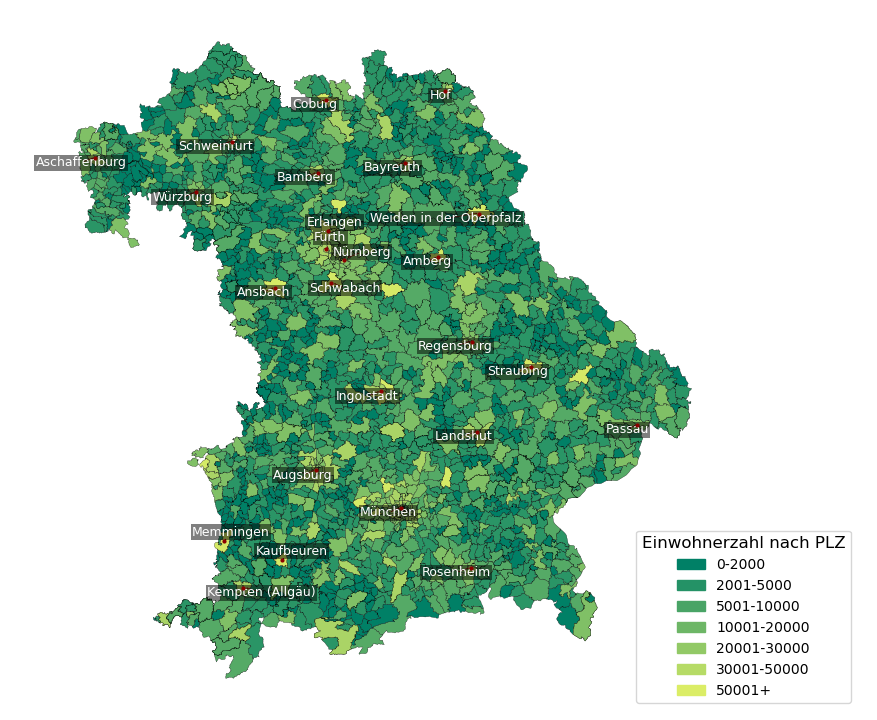
\includegraphics[width=0.95\textwidth]{figures/Bayern_pop_plz.png}
    \caption{Verteilung der Bevölkerungsdichte Bayerns nach Postleitzahlenbereichen. Quelle: Eigene Darstellung}
    \label{fig:bevoelkerungsdichte}
\end{figure}
\FloatBarrier



\subsubsection{Hochwassergeodaten}\label{sec:hochgeo}

Im Anschluss an die in Abschnitt \ref{sec:hypogeo} dargelegte Erfassung der geografischen Koordinaten der Hypothekendarlehen ergibt sich die Notwendigkeit einer weiterführenden Analyse. Diese zielt darauf ab, die räumliche Relation der betreffenden Immobilien zu den definierten Hochwasserrisikogebieten zu determinieren. Zur Durchführung dieser Analyse ist eine detaillierte Hochwasserrisikokarte für Bayern erforderlich.

Im Rahmen eines EU-weiten Stresstests stellt die \ac{EZB} den Banken zur Simulation eines schweren Überschwemmungsszenarios eine Hochwasserrisikokarte (Abbildung \ref{fig:euflut}) zur Verfügung.

\begin{figure}[htbp]
    \centering
    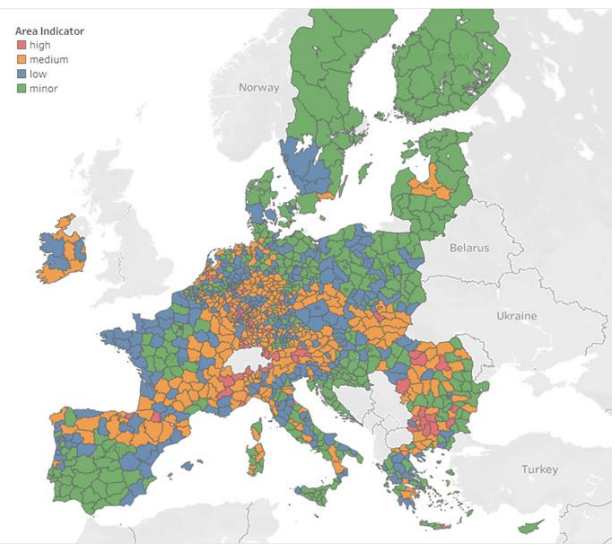
\includegraphics[width=0.6\textwidth]{figures/euflood.png} 
    \caption{EU-Hochwasserrisikokarte.Quelle: EZB 2022 Klimarisiko-Stresstest}
    \label{fig:euflut}
\end{figure}
\FloatBarrier

Die \ac{EZB}-Karte klassifiziert Regionen nach Hochwasserrisiken. Sie basiert auf Daten der Europäischen Kommission und Four Twenty Seven \parencite{ECB2022ClimateStressTest}. Allerdings sind die Basisdaten nicht öffentlich zugänglich. Zudem erlaubt die visuelle Darstellung keine präzise Identifikation spezifischer Gebiete. Folglich ergibt sich für Bayern die Notwendigkeit einer detaillierteren Analyse.

Die Kartierungen des Bayerischen Landesamts für Umwelt bieten eine fundierte Grundlage für die regionale Risikoanalyse. Diese für die Einzugsgebiete von Donau, Rhein und Elbe entwickelten Karten ermöglichen eine präzise Einschätzung der Hochwasserrisiken in Bayern \parencite{LfU_Bayern}. Sie visualisieren detailliert die Hochwassergefährdung, potenziell betroffene Landnutzungen und historische Hochwasserereignisse.
Diese Daten liegen im ETRS89-Koordinatensystem vor, während die Hypothekengeodaten das EPSG:3035-System nutzen. ETRS89 ist ein geodätisches Referenzsystem für Europa. Es misst Positionen in geografischen Koordinaten: Breitengrad und Längengrad. Diese werden in Grad, Minuten und Sekunden angegeben. ETRS89 bietet eine hohe Genauigkeit für kontinentale Messungen.
EPSG:3035 hingegen ist eine kartografische Projektion. Sie wandelt die Erdkrümmung in eine flache Ebene um. Positionen werden hier in Metern gemessen. X-Koordinaten repräsentieren den Abstand vom Projektionszentrum nach Osten. Y-Koordinaten messen den Abstand nach Norden. EPSG:3035 ist speziell für statistische Analysen in Europa konzipiert.
Zur Herstellung der Datenkohärenz erfolgt eine Koordinatentransformation in das EPSG:3035-System. 

\subsubsection{Überflutungstiefen}\label{sec:tief}
Die Schäden durch Überschwemmungen hängen von der Wassertiefe ab. Tieferes Wasser verursacht meist größere und teurere Schäden an Häusern. Für die Analyse der Überflutungstiefe in Bayern benötigt man Überflutungstiefen-Geodaten. \ac{DGM} Modell beschreibt die Höhe des Bodens, wobei eine hohe Auflösung genaue Ergebnisse liefert \parencite{vermessungsverwaltung2019gelandemodell}. Hochwasserstände aus Messungen sind wichtig für präzise Berechnungen. Dafür wurden Daten vom \textcite{bayern2016hochwassernachrichtendienst} für aktuelle Pegelstände betrachtet. Historische Hochwasserdaten helfen bei Einschätzungen künftiger Ereignisse und sind in Berichten und Karten enthalten. Diese wurden vom \textcite{LfU_Bayern} bezogen, wie in Abschnitt \ref{sec:hochgeo} beschrieben.
Die \ac{DGM}-Daten von \textcite{vermessungsverwaltung2019gelandemodell} für ganz Bayern umfassen ein sehr großes Datenvolumen von ca. 240 GB. Daher wurden nur Daten für die Gebiete mit Hypotheken-Datenpunkten aus Abschnitt \ref{sec:hypogeo} heruntergeladen.
Die Geländehöhe (m) für bestimmte Koordinaten wird aus dem Höhenraster, das aus der \ac{DGM}-Datei gelesen wurde, extrahiert.

Auf Grundlage der gesammelten Daten können die folgenden Berechnungen durchgeführt werden:
\begin{equation}
    \text{Absoluter Wasserstand (m)} = \text{Pegelnullpunkt (m)} + \left(\frac{\text{Pegelstand (cm)}}{100}\right)
\end{equation}

\begin{equation}
    \text{Hochwassertiefe (m)} = \max \left( \text{Wasserstand (m)} - \text{Geländehöhe (m)}, 0 \right)
\end{equation}
 Abbildung \ref{fig:ingolstadt} visualisiert das digitale Geländemodell für Ingolstadt, welches die topographischen Merkmale der Stadt und ihrer Umgebung detailliert darstellt und somit eine wichtige Grundlage für die Hochwasseranalyse bildet.
\begin{figure}[!ht]
    \centering
    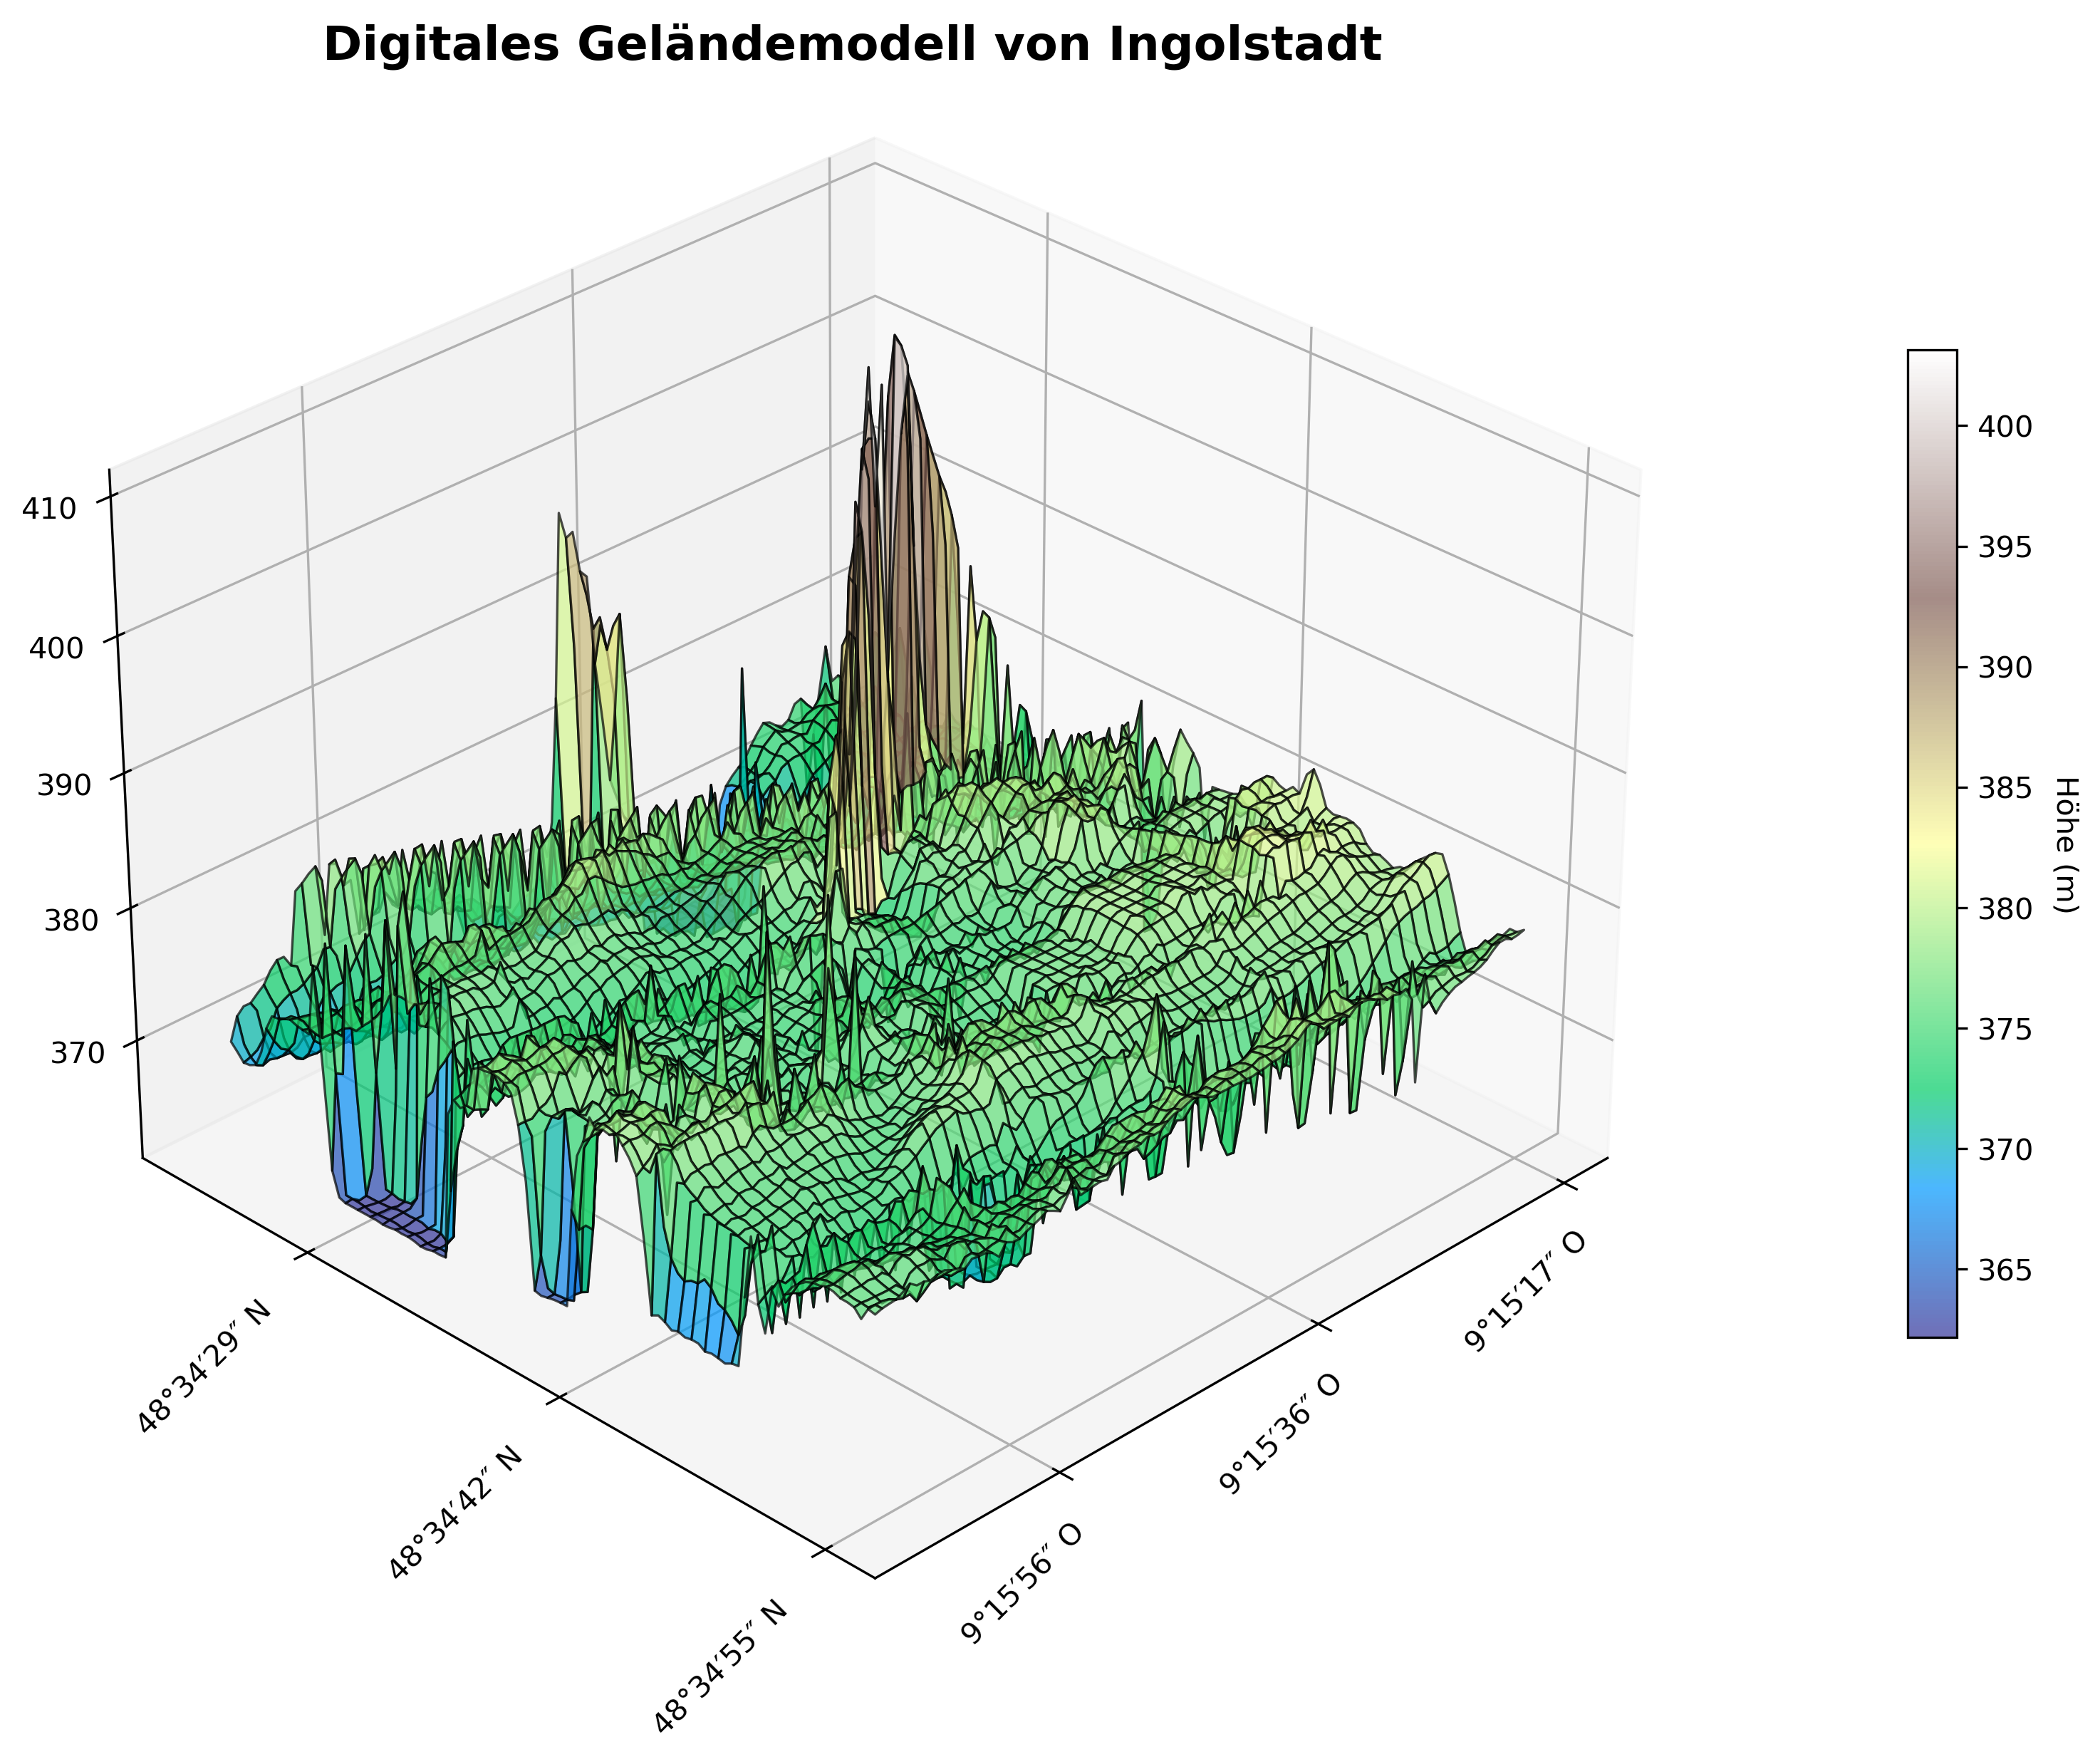
\includegraphics[width=0.8\textwidth]{figures/dgm_3d_wireframe_ingolstadt.png}
    \caption{Digital Geländemodell von Ingolstadt. Quelle: Eigene Darstellung}
    \label{fig:ingolstadt}
\end{figure}
\FloatBarrier
\subsection{Quadratmeterpreise}
Ein weiterer wichtiger Aspekt für ein realistisches Portfolio sind die Quadratmeterpreise. Die ungleiche Verteilung der Quadratmeterpreise ist allgemein bekannt. München gilt als die teuerste Stadt im Bundesland Bayern und in Deutschland und . Gemäß dem Bericht zum Immobilienmarkt liegen die Quadratmeterpreise für Eigenheime in der Stadt und im Landkreis München bei einem durchschnittlichen Preis von 10.200 EUR. In Kronach liegen die Preise bei 1.300 EUR \parencite{bayernlabo2024}. Es gibt große Varianz in den Preisen. Daher müssen die Darlehenspunkte an die jeweiligen Quadratmeterpreise des Standorts angeglichen werden. In Abbildung \ref{fig:preis} sind die Angebotspreise für Eigenheime in den bayerischen Landkreisen und kreisfreien Städten pro Quadratmeter in Euro dargestellt. Die Quadratmeterpreise für das Jahr 2023 wurden aufgeführt.
\begin{figure}[htbp]
    \centering
    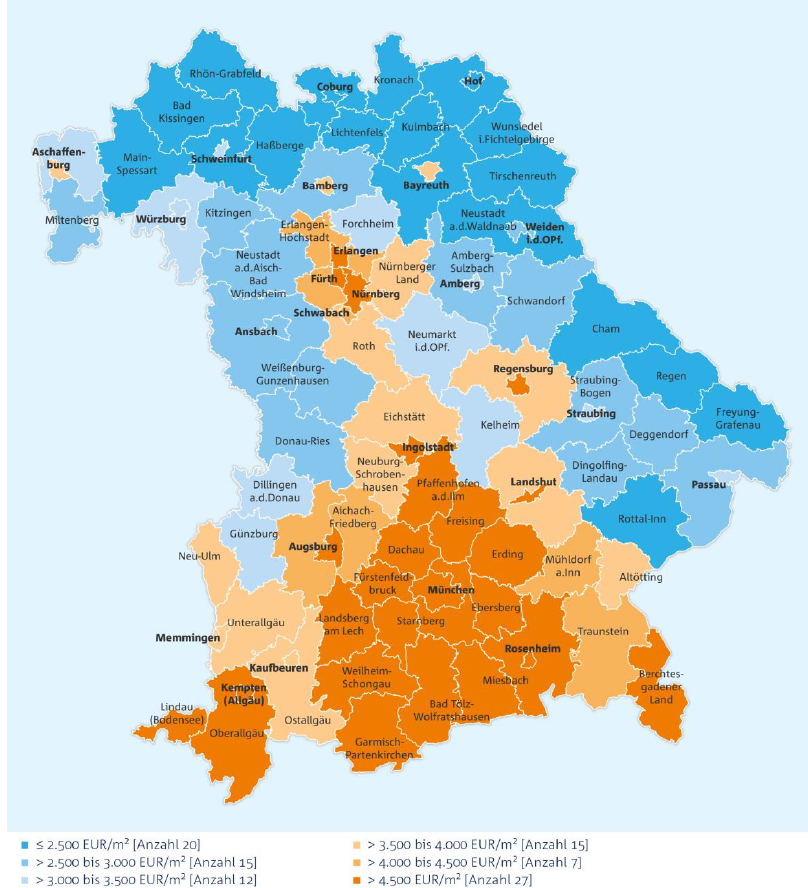
\includegraphics[width=0.8\textwidth]{figures/preism2.png}
    \caption{Angebotspreise 2023 in den bayerischen Landkreisen und kreisfreien Städten – Eigenheime – in €/m². Quelle: \textcite{bayernlabo2024} }
    \label{fig:preis}
\end{figure}
\FloatBarrier
\subsection{Verteilung der Energieeffizienzklassen in Bayern}
Wie bereits in Abschnitt \ref{sec:EPC} angegeben, haben Energieausweise für Wohngebäude einen direkten Einfluss auf die Betriebskosten und den Wert von Immobilien. Es gibt derzeit keine offiziellen Statistiken von staatlichen Behörden über die Verteilung von Energieeffizienzklassen in Bayern. Laut McMaker, einem führenden Maklerunternehmen in Deutschland, liegt Bayern jedoch an erster Stelle bei Wohnimmobilien mit positiven Energiekennwerten. In Bayern sind etwa 18\% der Wohnimmobilien energieeffizient (A+, A oder B), während 36\% schlechte Energiekennwerte haben \parencite{mcmakler2022}. Der Grund dafür liegt darin, dass die durchschnittliche Wohnimmobilie in Bayern erst 1991 gebaut wurde, was einen großen Unterschied im Vergleich zu anderen Bundesländern darstellt. Tabelle \ref{tab:epc_bayern} zeigt die Verteilung der Energieeffizienzklassen in Bayern.
\begin{table}[htbp]
    \centering
    \caption{Prozentuale Verteilung der Energieeffizienzklassen in Bayern}
    \label{tab:epc_bayern}
    \begin{tabularx}{\textwidth}{>{\raggedright\arraybackslash}X >{\centering\arraybackslash}X >{\centering\arraybackslash}X >{\centering\arraybackslash}X}
        \toprule
        & \textbf{A+, A, B} & \textbf{C, D, E} & \textbf{F, G, H} \\
        \midrule
        \textbf{Prozentanteil} & 18\% & 46\% & 36\% \\
        \bottomrule
    \end{tabularx}
\end{table}

Durch die Anwendung dieser Verteilung kann die \ac{EPC}-Verteilung in unser Hypothekenportfolio integriert werden, um eine möglichst realistische Darstellung des Portfolios zu erreichen.



\subsection{Übersicht über das Hypothekenportfolio}
Nachdem alle genannten Schritte der Datenanalyse abgeschlossen waren, wurde ein realistisches Portfolio von Hypotheken-Immobilien erstellt. Die in Tabelle \ref{tab:objekt-variablen} beschriebenen Objektvariablen bilden die Grundlage. Sie dienen der Berechnung physischer Risiken und Transitionsrisiken im nächsten Abschnitt.
\begin{table}[htbp]
    \centering
    \small
    \caption{Übersicht über das Hypothekenportfolio und die relevanten Objekt-Variablen}
    \label{tab:objekt-variablen}
    \begin{tabularx}{1.0\textwidth}{>{\raggedright\arraybackslash}X >{\raggedright\arraybackslash}X}
        \toprule
        \textbf{Objekt-Variablen} & \textbf{Erklärung} \\
        \midrule
        ID & Identifikationsnummer \\
        \addlinespace
        Ort & Ort der Immobilie \\
        \addlinespace
        Landkreis & Landkreis der Immobilie \\
        \addlinespace
        Geometrie & Geometrische Lage der Immobilie, bestehend aus Breiten- und Längengrad zur Berechnung der Überschwemmungsgefahr an diesem Punkt \\
        \addlinespace
        GEB\_Q & Hochwasser Ergeiniss \\
        \addlinespace
        Überschwemmung Tiefe & Tiefe der Überschwemmung an dem Punkt \\
        \addlinespace
        Überschwemmungsrisiko Stufe & Stufe des Überschwemmungsrisikos \\
        \addlinespace
        Energieklasse & Energieeffizienzklasse der Immobilie \\
        \addlinespace
        Aktueller Immobilienwert & Der aktuelle Wert der Immobilie \\
        \addlinespace
        Aktuelles LTV & Aktuelles Verhältnis von Darlehen zu Wert (Loan-to-Value) \\

        \bottomrule
    \end{tabularx}
\end{table}



\clearpage

\section{Modellierungstruktur}
\subsection{Modellierung des Hochwasserrisikos}
In diesem Abschnitt wird bei der Modellierung des Hochwasserrisikos die grundlegende Quantifizierung des physischen Risikos erläutert.
\subsubsection{Schadensfunktion}
Wie bereits in Abschnitt \ref{sec:tief} erwähnt, hängen die Schäden durch Überschwemmungen von der Wassertiefe ab. In diesem Abschnitt wird erklärt, wie diese Abhängigkeit konkret besteht.
Sobald verschiedene Flutwassertiefen ermittelt sind, wird eine spezifische Schadensfunktion für Wohnimmobilien \acs{RRE} entwickelt. Diese basiert auf der Methodik des Gemeinsamen Forschungszentrums \acs{JRC} der Europäischen Union \parencite{huizinga2017global}.

Da die Studie von \textcite{huizinga2007flood} unveröffentlicht ist, können die Daten nur aus den Diagrammen zur Schadensberechnung pro Quadratmeter und Schadensfaktor für verschiedene Regionen entnommen werden.

Abbildung \ref{fig:damage_curve1} und \ref{fig:damage_curve2} präsentieren zwei Grafiken, die die Schadenshöhe pro Quadratmeter und den Schadensfaktor für unterschiedliche europäische Regionen veranschaulichen.

\begin{figure}[H]
    \centering
    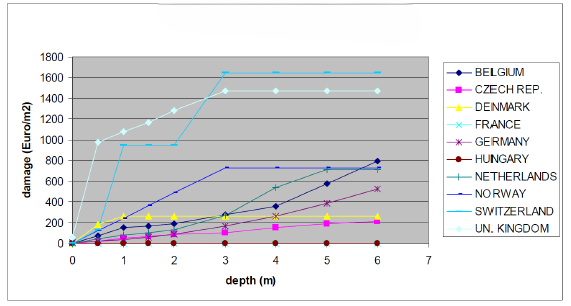
\includegraphics[width=0.8\textwidth]{figures/RREdamagem2.png}
    \caption{Schaden pro Quadratmeter in verschiedenen Regionen Europas. Quelle: J. Huizinga und al., 2017}
    \label{fig:damage_curve1}
\end{figure}

\begin{figure}[H]
    \centering
    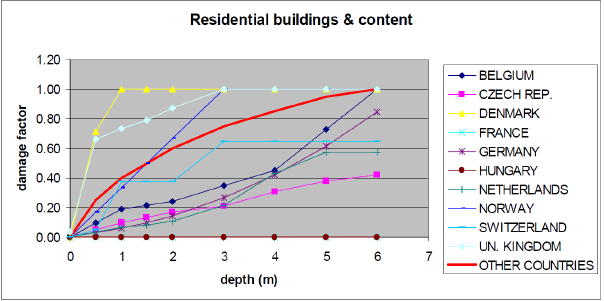
\includegraphics[width=0.8\textwidth]{figures/RREdamage.png}
    \caption{Schadensfaktor für Wohnimmobilien in verschiedenen Regionen Europas. Quelle: J. Huizinga und al., 2017}
    \label{fig:damage_curve2}
\end{figure}
\subsubsection{Berechnung von Hochwasserschäden}
Gemäß der Definition von der \textcite{undro1979,} ergibt sich das Risiko aus drei Komponenten: Gefährdungswahrscheinlichkeit,  den betroffenen Elemente (Exposition) und Vulnerabilität. \parencite{coburn1991vulnerability}. Dies kann vereinfacht ausgedrückt werden als:

\begin{equation}
    \text{Physisches Risiko} = \text{Gefährdungswahrscheinlichkeit} \times \text{Exposition} \times \text{Vulnerabilität}
\end{equation}

Um eine genauere Analyse der einzelnen Immobilienschäden zu ermöglichen, wird eine detailliertere Schadensformel \parencite{vanweddingen2023physicalrisk} benutzt:
\begin{equation}
    Immobilienschaden_{i,j} = E_j \times d(I_{i,j}|v_j)
    \label{eq:schaden}
\end{equation}
Wobei:
\begin{itemize}
    \item i das spezifische Ereignis bezeichnet
    \item $E_j$ den Wert der einzelnen Immobilie am Standort j repräsentiert
    \item $d$ die spezifische Schadensfunktion darstellt
    \item $I_{i,j}$ die lokale Intensität des Ereignisses i am Standort j ist
    \item $v_j$ die spezifische Vulnerabilität der einzelnen Immobilie am Standort j bezeichnet
\end{itemize}

Formel \ref{eq:schaden} berücksichtigt die Gefährdungswahrscheinlichkeit nicht, da sie den Schaden für ein einzelnes Ereignis berechnet. Für den erwarteten jährlichen Immobilienschaden wird die jährliche Überschreitungswahrscheinlichkeit aus Kapitel \ref{sec:EPC} benötigt und wird nachfolgend berechnet:
\begin{equation}
    EAI_j = \sum_i Immobilienschaden_{i,j} \times p(I_{i,j})
    \label{eq:EAI}
\end{equation}
Hierbei steht \acs{EAI} für den erwarteten jährlichen Schaden, und \( p(I_{i,j}) \) ist die Eintrittswahrscheinlichkeit des Ereignisses \( i \) mit der Intensität \( I_{i,j} \) am Standort \( j \).
Auf Grundlage der Formel \ref{eq:EAI} wird der erwartete Einfluss \acs{EI}, über die Kreditlaufzeit wie folgt berechnet:
\begin{equation}
    EI(j) = EAI(j) \times T
\end{equation}
Dabei ist \( EI(j) \) der gesamte erwartete Schaden über die Kreditlaufzeit \( T \).

Die Auswirkungen auf den Immobilienwert nach einem Schaden werden wie folgt berechnet:
\begin{equation}
    \text{Neuer Immobilienwert} = \text{Ursprünglicher Immobilienwert} - \text{Schaden}
\end{equation}

Zur Bestimmung der neuen Beleihungsquote \ac{LtV} auf Basis des angepassten Immobilienwertes gilt:
\begin{equation}
    \text{Neue LtV} = \frac{\text{Darlehenbetrag}}{\text{Neuer Immobilienwert}}
\end{equation}

Die risikogewichteten Aktiva \acs{RWA}, abhängig von der Beleihungsquote, berechnen sich folgendermaßen:
\begin{equation}
    RWA = \text{Darlehenbetrag} \times \text{Risikogewicht}
\end{equation}
Das Risikogewicht wird anhand der Beleihungsquote ermittelt.

Zum Schluss lässt sich die prozentuale Änderung der \acs{RWA} mit dieser Formel bestimmen:
\begin{equation}
    \% \text{Änderung RWA} = \frac{\text{Neue RWA}}{\text{Ursprüngliche RWA}} - 1
\end{equation}



\clearpage
\printbibliography[title=Literaturverzeichnis,heading=bibintoc]

\clearpage
% cSpell:disable
\section*{Selbstständigkeitserklärung}

\begin{flushleft}
Hiermit erkläre ich, dass ich die vorliegende Arbeit selbstständig und ohne fremde Hilfe verfasst und keine anderen Hilfsmittel als die angegebenen verwendet habe.

\vspace{2em}

München, den \today

\vspace{2em}


\includegraphics[width=0.17\textwidth]{logos/signature.png}
\end{flushleft}

\end{document}